\chapter{Support Vector Machines}\label{ch-13}

\textbf{Support Vector Machines} (SVMs) are the answer to the question
left open by SLT
(\href{12\%20-\%20Statistical\%20Learning\%20Theory\%20e\%20VC-dimension}{12
- Statistical Learning Theory and VC-dimension}): is it possible to fix
the training error and \textbf{automatically} minimise the
VC-confidence? The SVM is still a linear machine (an LTU), but among
all separating hyperplanes it chooses the one that \textbf{maximises
the margin}, and this is equivalent to controlling the VC-dimension.
The lecture proceeds in four steps: linear \emph{hard margin} SVM,
\emph{soft margin} SVM for non-separable data, \textbf{kernels} for
non-linear problems, and finally SVM for \textbf{regression}.

\begin{boxnote}{Notation (from Haykin, ch.\ 6)}

\(N\) is the number of examples (previously \(l\)), with indices \(i\)
and \(j\) for the patterns; \(m\) is the dimension of the input vector
(previously \(n\)); \(b\) is used instead of \(w_0\) for the bias. The
parts marked with * in the slides are useful for completeness but not
essential for using the model (and for a standard oral exam): in
particular the details of the solution with Lagrange multipliers.

\end{boxnote}

\section{Part I --- SVM for binary
classification}\label{parte-i-svm-per-la-classificazione-binaria}

An SVM is:

\begin{itemize}
\tightlist
\item
  a \textbf{linear machine} (like the LTU or the Perceptron);
\item
  that \textbf{maximises the separation margin};
\item
  and implements \textbf{Structural Risk Minimization}.
\end{itemize}

Initially (\emph{hard margin} SVM) the problem is assumed to be
\textbf{linearly separable} and the data are assumed to contain
\textbf{no errors}.

\begin{figure}[htbp]
\centering
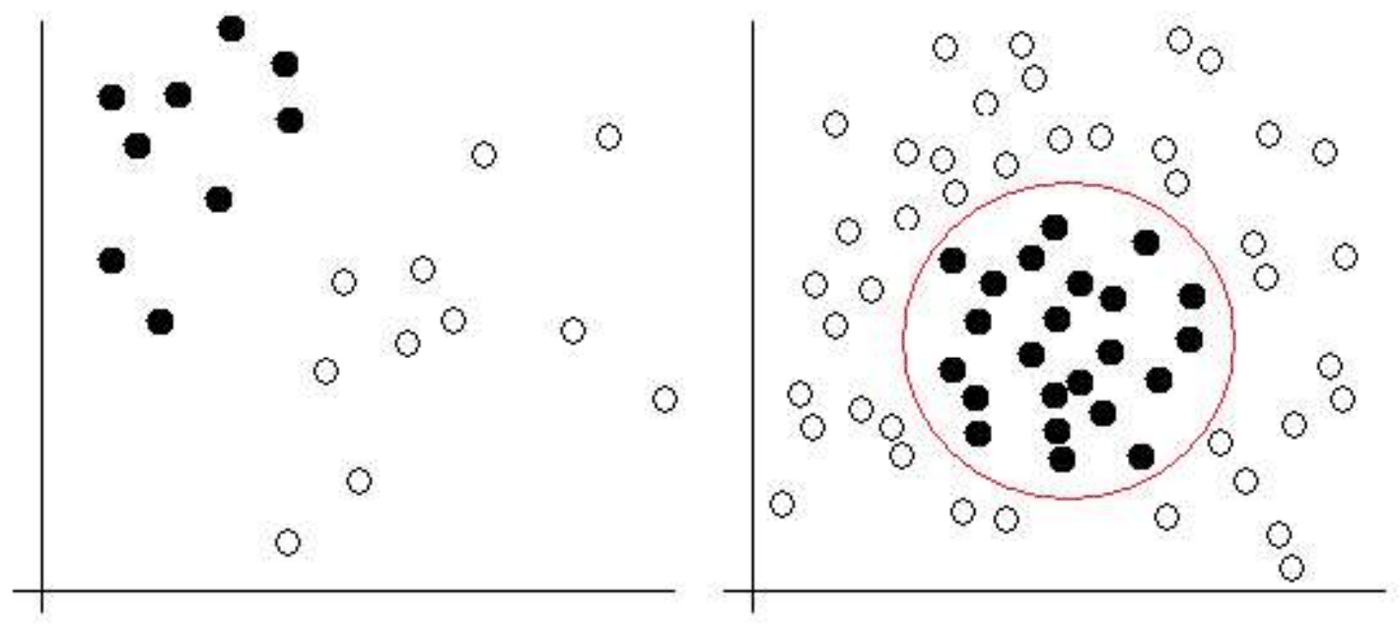
\includegraphics[width=0.71\linewidth,height=0.42\textheight,keepaspectratio]{images/13-svm_separabili.png}
\caption{Linearly separable (left) and non-linearly separable (right)
patterns.}
\end{figure}

\subsection{The separating hyperplane}\label{liperpiano-separatore}

Given the training set \(T = \{(\mathbf{x}_i, d_i)\}_{i=1}^{N}\), we
look for a hyperplane \(\mathbf{w}^T\mathbf{x} + b = 0\) that separates
the examples: \[
\mathbf{w}^T\mathbf{x}_i + b \ge 0 \;\text{ if } d_i = +1, \qquad \mathbf{w}^T\mathbf{x}_i + b < 0 \;\text{ if } d_i = -1.
\] \(g(\mathbf{x}) = \mathbf{w}^T\mathbf{x} + b\) is the
\textbf{discriminant function} and
\(h(\mathbf{x}) = \operatorname{sign}(g(\mathbf{x}))\) is the
\textbf{hypothesis}.

\subsection{The separation margin}\label{il-margine-di-separazione}

\begin{boxdefinition}{Separation margin}

If the hyperplane is at the same distance from the nearest positive
example and from the nearest negative one, the \textbf{separation
margin} \(\rho\) is twice the distance between the hyperplane and the
nearest point. It can be thought of as a \textbf{``safety zone''}
around the boundary.

\end{boxdefinition}

\begin{figure}[htbp]
\centering
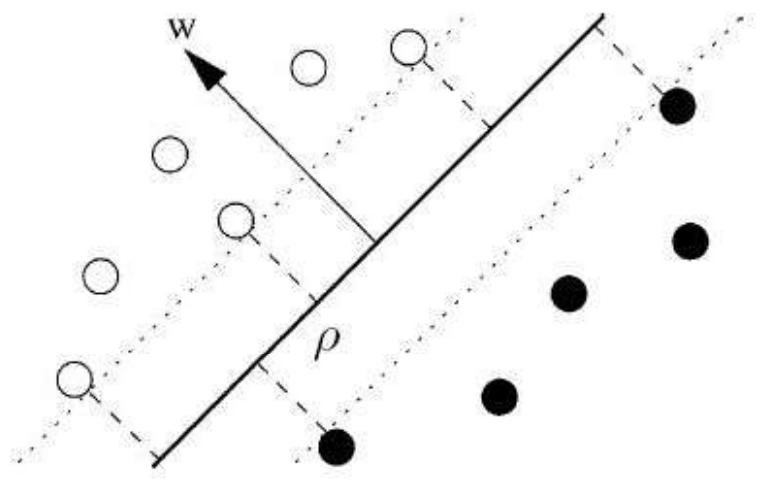
\includegraphics[width=0.43\linewidth,height=0.42\textheight,keepaspectratio]{images/13-svm_margine.png}
\caption{The separation margin \(\rho\).}
\end{figure}

Not all hyperplanes that solve the problem are equal: as the separating
hyperplane varies, the margin varies too.

\begin{figure}[htbp]
\centering
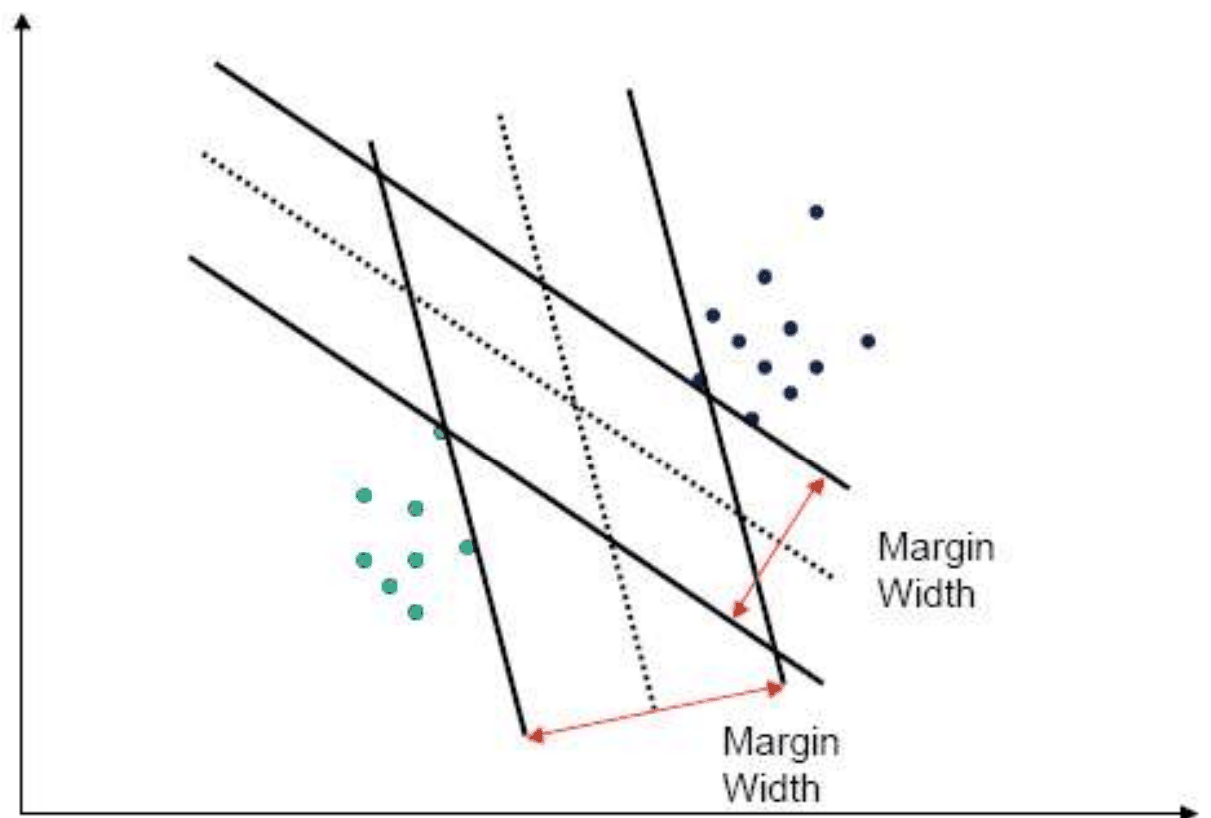
\includegraphics[width=0.60\linewidth,height=0.42\textheight,keepaspectratio]{images/13-svm_margini-diversi.png}
\caption{Different separating hyperplanes have different margins.}
\end{figure}

\begin{boxdefinition}{Optimal hyperplane}

The \textbf{optimal hyperplane} \(\mathbf{w}_o^T\mathbf{x} + b_o = 0\)
(``o'' stands for \emph{optimal}) is the one that \textbf{maximises the
margin} \(\rho\). We will see that \(\rho = \dfrac{2}{\|\mathbf{w}\|}\),
hence \[
\text{maximising } \rho \iff \text{minimising } \|\mathbf{w}\|.
\]

\end{boxdefinition}

\subsection{Canonical representation and support
vectors}\label{rappresentazione-canonica-e-support-vector}

Thanks to \textbf{scale freedom} (multiplying \(\mathbf{w}\) and \(b\)
by a constant does not change the hyperplane) we can rescale
\(\mathbf{w}\) and \(b\) so that the points closest to the hyperplane
satisfy \(|g(\mathbf{x}_i)| = |\mathbf{w}^T\mathbf{x}_i + b| = 1\).
Then: \[
\mathbf{w}^T\mathbf{x}_i + b \ge 1 \;\text{ if } d_i = +1, \qquad \mathbf{w}^T\mathbf{x}_i + b \le -1 \;\text{ if } d_i = -1,
\] i.e., in compact form: \[
d_i(\mathbf{w}^T\mathbf{x}_i + b) \ge 1 \qquad \forall i = 1,\dots,N.
\]

\begin{boxdefinition}{Support vector}

A \textbf{support vector} \(\mathbf{x}^{(s)}\) satisfies the constraint
\textbf{with equality}: \(d^{(s)}(\mathbf{w}^T\mathbf{x}^{(s)} + b) = 1\).
Support vectors are the points \textbf{closest} to the hyperplane, those
lying on the edge of the margin.

\end{boxdefinition}

\begin{figure}[htbp]
\centering
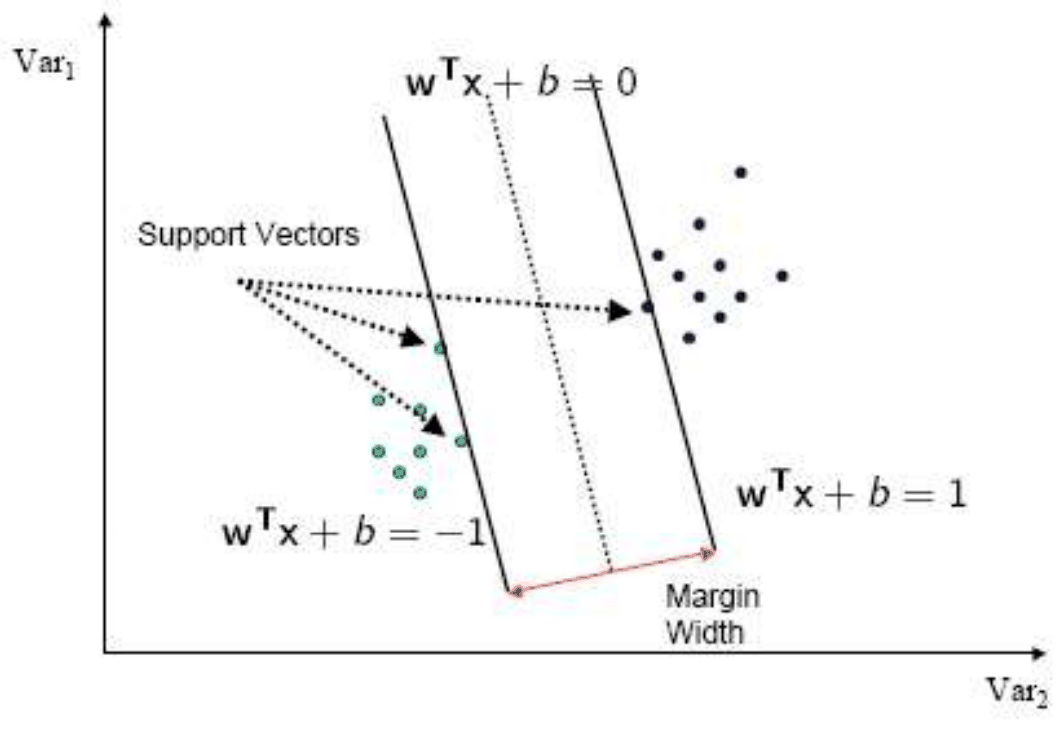
\includegraphics[width=0.60\linewidth,height=0.42\textheight,keepaspectratio]{images/13-svm_support-vectors.png}
\caption{Support vectors lie on the lines
\(\mathbf{w}^T\mathbf{x} + b = \pm 1\).}
\end{figure}

\subsection{Computing the margin}\label{calcolo-del-margine}

\textbf{Distance of a point from the hyperplane.} Let \(r\) be the
distance between \(\mathbf{x}\) and the optimal hyperplane. Since
\(\mathbf{w}_o\) is orthogonal to the hyperplane, we can write \[
\mathbf{x} = \mathbf{x}_p + r\,\frac{\mathbf{w}_o}{\|\mathbf{w}_o\|},
\] where \(\mathbf{x}_p\) is the projection of \(\mathbf{x}\) onto the
hyperplane.

\begin{figure}[htbp]
\centering
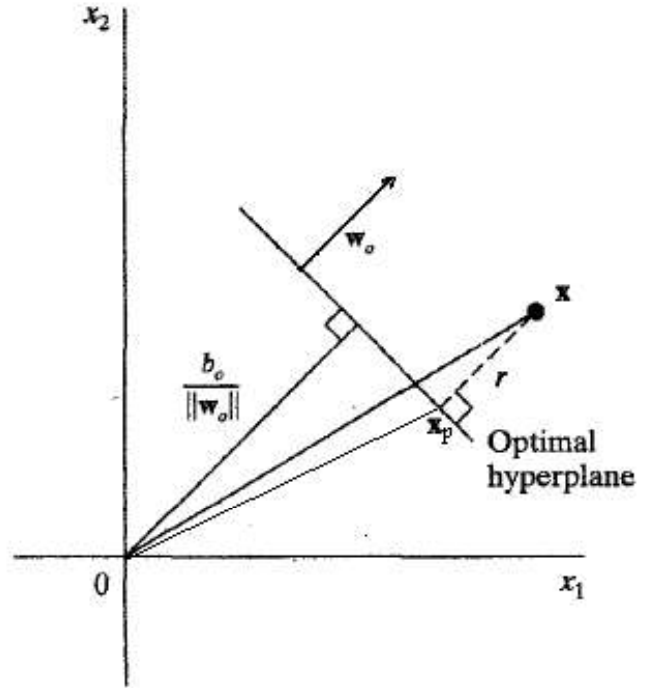
\includegraphics[width=0.43\linewidth,height=0.42\textheight,keepaspectratio]{images/13-svm_distanza.png}
\caption{Distance \(r\) between a point \(\mathbf{x}\) and the optimal
hyperplane.}
\end{figure}

Evaluating \(g(\mathbf{x}) = \mathbf{w}_o^T\mathbf{x} + b_o\): \[
g(\mathbf{x}) = \mathbf{w}_o^T\mathbf{x}_p + b_o + r\,\mathbf{w}_o^T\frac{\mathbf{w}_o}{\|\mathbf{w}_o\|} = \underbrace{g(\mathbf{x}_p)}_{=0} + r\,\frac{\|\mathbf{w}_o\|^2}{\|\mathbf{w}_o\|} = r\,\|\mathbf{w}_o\|,
\] because \(\mathbf{x}_p\) lies on the hyperplane. Hence \[
r = \frac{g(\mathbf{x})}{\|\mathbf{w}_o\|}.
\]

\textbf{Margin.} For a positive support vector
\(g(\mathbf{x}^{(s)}) = 1\), so its distance from the hyperplane is
\(r = \frac{1}{\|\mathbf{w}_o\|} = \frac{\rho}{2}\). Hence: \[
\rho = \frac{2}{\|\mathbf{w}_o\|}.
\] The optimal hyperplane maximises \(\rho\), i.e.\ it
\textbf{minimises \(\|\mathbf{w}\|\)}.

\subsection{The quadratic optimisation problem (hard
margin)}\label{il-problema-di-ottimizzazione-quadratica-hard-margin}

The formal derivation requires \textbf{constrained optimisation}
techniques (assumed known, for example from the CM course); quadratic
programming is considered solved by existing packages. Here we are
interested in understanding how the problem is formulated, the
relationship between support vectors and multipliers \(\alpha\), and
the final result for \(\mathbf{w}_o\).

\begin{boxdefinition}{Primal problem --- hard margin SVM}

Given \(T = \{(\mathbf{x}_i, d_i)\}_{i=1}^N\), find \(\mathbf{w}\) and
\(b\) that minimise \[
\Psi(\mathbf{w}) = \frac{1}{2}\mathbf{w}^T\mathbf{w} \qquad (\text{i.e. } \min \|\mathbf{w}\|)
\] subject to the constraints (zero classification errors) \[
d_i(\mathbf{w}^T\mathbf{x}_i + b) \ge 1 \qquad \forall i = 1,\dots,N.
\]

\end{boxdefinition}

\begin{itemize}
\tightlist
\item
  The objective function is \textbf{quadratic and convex} in
  \(\mathbf{w}\).
\item
  The constraints are \textbf{linear} in \(\mathbf{w}\).
\item
  Solving this problem scales with the dimension of the input space
  \(m\) (the actual cost depends anyway on the solver algorithm).
\end{itemize}

\subsubsection{Solution with Lagrange
multipliers*}\label{soluzione-con-i-moltiplicatori-di-lagrange}

The \textbf{Lagrangian} is built: \[
J(\mathbf{w}, b, \boldsymbol{\alpha}) = \frac{1}{2}\mathbf{w}^T\mathbf{w} - \sum_{i=1}^{N}\alpha_i\big(d_i(\mathbf{w}^T\mathbf{x}_i + b) - 1\big),
\] with \(\alpha_i \ge 0\) the \textbf{Lagrange multipliers}, one for
each constraint of the primal. \(J\) must be \textbf{minimised with
respect to \(\mathbf{w}\) and \(b\)} and \textbf{maximised with respect
to \(\boldsymbol{\alpha}\)}: the solution is a \textbf{saddle point} of
\(J\).

Optimality conditions: \[
\frac{\partial J}{\partial \mathbf{w}} = 0 \;\Rightarrow\; \mathbf{w} = \sum_{i=1}^{N}\alpha_i d_i\mathbf{x}_i, \qquad \frac{\partial J}{\partial b} = 0 \;\Rightarrow\; \sum_{i=1}^{N}\alpha_i d_i = 0.
\]

\textbf{Kuhn-Tucker conditions.} At the saddle point \[
\alpha_i\big(d_i(\mathbf{w}^T\mathbf{x}_i + b) - 1\big) = 0 \qquad \forall i.
\] Therefore:

\begin{itemize}
\tightlist
\item
  if \(\alpha_i > 0\), then \(d_i(\mathbf{w}^T\mathbf{x}_i + b) = 1\):
  \(\mathbf{x}_i\) is a \textbf{support vector};
\item
  if \(\mathbf{x}_i\) is not a support vector, then \(\alpha_i = 0\).
\end{itemize}

\begin{boxtip}{The hyperplane depends only on the support vectors}

\(\mathbf{w}_o = \sum_{i=1}^{N_s}\alpha_{o,i}\,d_i\,\mathbf{x}_i\): the
sum is restricted to the \(N_s\) support vectors. \textbf{The
hyperplane depends only on the support vectors!} All the other points
could be removed without changing the solution.

\end{boxtip}

\subsubsection{The dual problem*}\label{il-problema-duale}

Substituting the optimality conditions into \(J\) we obtain the
\textbf{dual problem}, in which only the multipliers appear:

\begin{boxdefinition}{Dual problem --- hard margin SVM}

Find \(\{\alpha_i\}_{i=1}^N\) that maximise \[
Q(\boldsymbol{\alpha}) = \sum_{i=1}^{N}\alpha_i - \frac{1}{2}\sum_{i=1}^{N}\sum_{j=1}^{N}\alpha_i\alpha_j d_i d_j\,\mathbf{x}_i^T\mathbf{x}_j
\] subject to \(\alpha_i \ge 0\) for all \(i\) and
\(\sum_{i=1}^{N}\alpha_i d_i = 0\).

\end{boxdefinition}

The \(\alpha\) are found by solving the \textbf{quadratic programming}
(QP) problem or with more recent and efficient approaches (for example
\textbf{SMO}, \emph{Sequential Minimal Optimization}). The dual scales
with the \textbf{number of examples \(N\)}, less with the dimension of
the space. Note that the data appear \textbf{only through dot products}
\(\mathbf{x}_i^T\mathbf{x}_j\): this will be the key to kernels.

\subsubsection{\texorpdfstring{Obtaining \(\mathbf{w}_o\) and
\(b_o\)}{Obtaining \textbackslash mathbf\{w\}\_o and b\_o}}\label{ottenere-mathbfw_o-e-b_o}

\begin{enumerate}
\def\labelenumi{\arabic{enumi}.}
\tightlist
\item
  Solve the dual obtaining \(\{\alpha_{o,i}\}\).
\item
  Compute \(\mathbf{w}_o = \sum_{i=1}^N\alpha_{o,i}d_i\mathbf{x}_i\).
\item
  Compute \(b_o = 1 - \mathbf{w}_o^T\mathbf{x}^{(s)}\) for a positive
  support vector \(\mathbf{x}^{(s)}\), i.e.\
  \(b_o = 1 - \sum_{i=1}^N\alpha_{o,i}d_i\,\mathbf{x}_i^T\mathbf{x}^{(s)}\).
\end{enumerate}

\subsection{How it is used}\label{come-si-usa}

There is no need to know \(\mathbf{w}_o\) explicitly: the multipliers
(from the dual) and the bias are enough. The decision surface is \[
\mathbf{w}_o^T\mathbf{x} + b_o = 0 \iff \sum_{i=1}^N\alpha_{o,i}\,d_i\,\underbrace{\mathbf{x}_i^T\mathbf{x}}_{\text{dot product}} + b_o = 0.
\] Given a pattern \(\mathbf{x}\): (1) compute
\(g(\mathbf{x}) = \sum_{i=1}^N\alpha_{o,i}d_i\,\mathbf{x}_i^T\mathbf{x} + b_o\);
(2) classify with the sign of \(g(\mathbf{x})\). The sum can be
restricted to the \(N_s\) support vectors.

\subsection{Why does it improve
generalisation?}\label{perchuxe9-migliora-la-generalizzazione}

On linearly separable problems we have \textbf{fixed the training
error} (at zero). Minimising the norm of \(\mathbf{w}\) is then
equivalent to \textbf{minimising the VC-dimension}, and hence the
capacity term (VC-confidence) \(\varepsilon\) in \[
R[h] \le R_{emp}[h] + \varepsilon(VC, N, \delta).
\]

\begin{boxtheorem}{Vapnik's theorem}

Let \(D\) be the diameter of the smallest sphere containing the data
\(\mathbf{x}_1,\dots,\mathbf{x}_N\). For the class of separating
hyperplanes \(\mathbf{w}^T\mathbf{x} + b = 0\) with margin \(\rho\),
the VC-dimension is bounded by \[
VC \le \min\left(\left\lceil\frac{D^2}{\rho^2}\right\rceil, m_0\right) + 1.
\]

\end{boxtheorem}

Since \(\frac{D^2}{\rho^2} \propto \text{Radius}^2\,\|\mathbf{w}\|^2\),
the VC-dim can be \textbf{smaller than \(m_0 + 1\)} (that of generic
hyperplanes) by restricting the search to ``regularised'' hyperplanes
with maximum margin. \textbf{The larger the margin, the smaller the
VC-dim}, regardless of the dimension of the space.

\subsection{Why it is an elegant
approach}\label{perchuxe9-uxe8-un-approccio-elegante}

For linearly separable data there are many solutions; Vapnik proposes
the maximum-margin \textbf{optimal separating hyperplane}, which
provides:

\begin{itemize}
\tightlist
\item
  a \textbf{unique solution} (unlike the iterative Perceptron
  algorithm) with \textbf{zero errors} (unlike LMS) for the binary
  classifier;
\item
  an \textbf{automated SRM}, which minimises the VC-confidence (by
  maximising the margin) directly within the optimisation process,
  \textbf{without hyperparameters} in the separable case;
\item
  the use of \textbf{constrained quadratic programming} solvers
  (instead of gradient descent), with a nice dual form that shows the
  support vectors and the dot products between patterns;
\item
  a solution focused on \textbf{``selected''} training data, the
  support vectors: a strength, because it does not depend on points far
  from the boundary; a weakness, because one hopes that the points on
  the boundary are not the noisiest.
\end{itemize}

But what to do with \textbf{noisy} or \textbf{non-linearly separable}
data?

\section{Soft margin SVM: allowing
errors}\label{svm-soft-margin-ammettere-errori}

If at least one point violates the exact separation condition
\(d_i(\mathbf{w}^T\mathbf{x}_i + b) \ge 1\), we move to the \textbf{soft
margin}.

\begin{figure}[htbp]
\centering
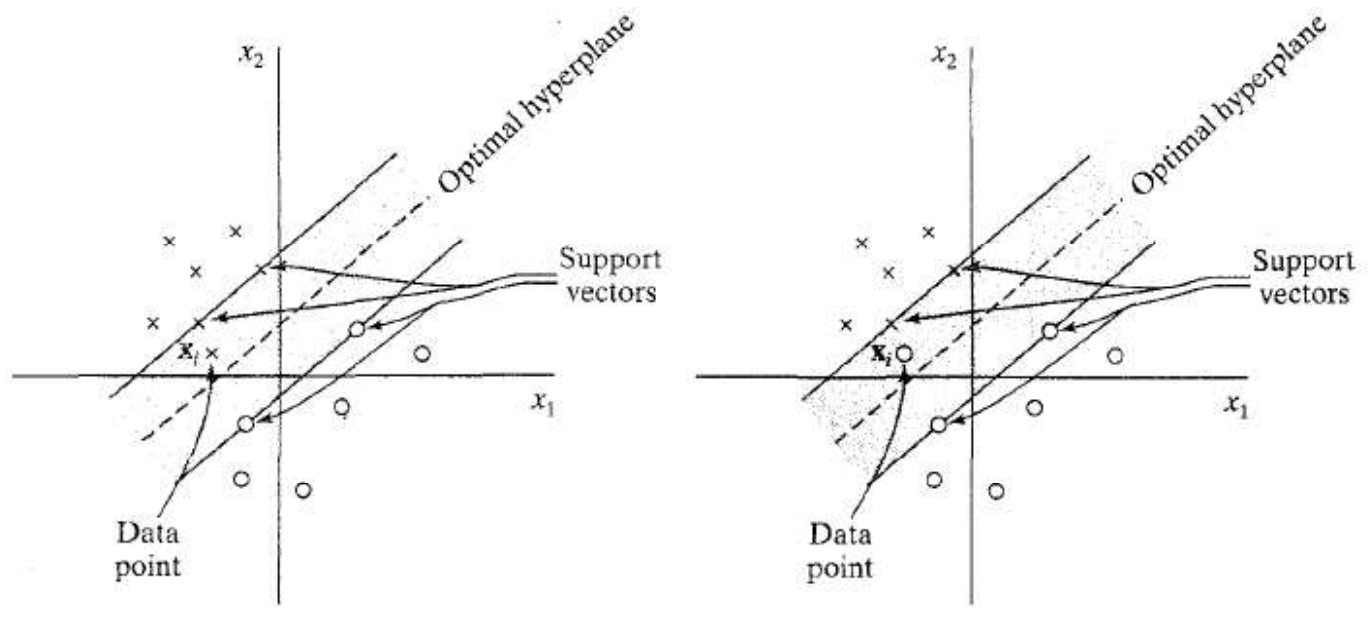
\includegraphics[width=0.71\linewidth,height=0.42\textheight,keepaspectratio]{images/13-svm_soft-margin.png}
\caption{Patterns violating the margin, without (left) and with (right)
classification error.}
\end{figure}

\begin{boxtip}{The advantage of the soft margin}

Allowing points inside the margin makes it possible to have a
\textbf{wider margin}: one obtains noise tolerance and a simpler model.
(Exercise: find the margin in the figures without allowing points
inside it.)

\end{boxtip}

\subsection{Slack variables}\label{variabili-slack}

Non-negative variables \(\xi_i \ge 0\), called \textbf{slack
variables}, are introduced, and the constraints become \[
d_i(\mathbf{w}^T\mathbf{x}_i + b) \ge 1 - \xi_i \qquad \forall i.
\] - \(\xi_i = 0\): the point is outside the margin or on its edge; -
\(0 < \xi_i \le 1\): the point is inside the margin but correctly
classified; - \(\xi_i > 1\): the point is misclassified.

A support vector now satisfies
\(d_i(\mathbf{w}^T\mathbf{x}_i + b) = 1 - \xi_i\).

\begin{figure}[htbp]
\centering
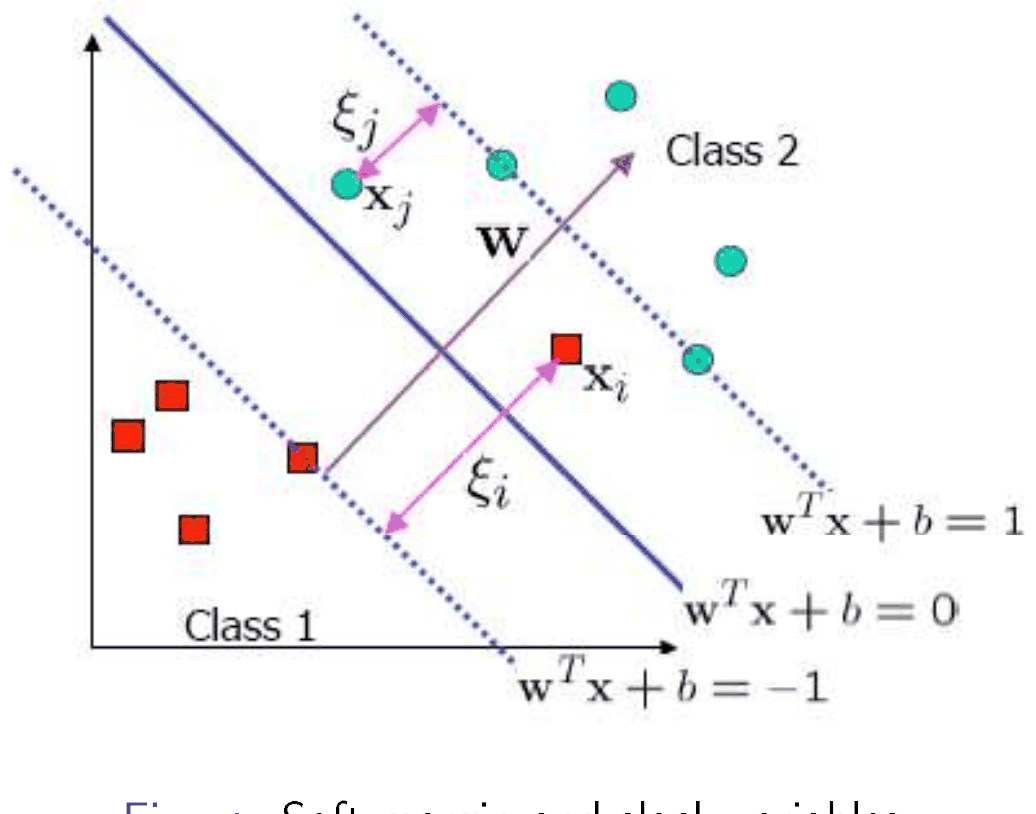
\includegraphics[width=0.54\linewidth,height=0.42\textheight,keepaspectratio]{images/13-svm_slack.png}
\caption{Soft margin and slack variables.}
\end{figure}

Beware: \textbf{Vapnik's theorem no longer holds} (the hard margin does
not allow points inside the margin).

\subsection{The soft margin primal
problem}\label{il-problema-primale-soft-margin}

\begin{boxdefinition}{Primal problem --- soft margin SVM}

Find \(\mathbf{w}\) and \(b\) that minimise \[
\Psi(\mathbf{w}, \boldsymbol{\xi}) = \frac{1}{2}\mathbf{w}^T\mathbf{w} + C\sum_{i=1}^{N}\xi_i
\] subject to \(d_i(\mathbf{w}^T\mathbf{x}_i + b) \ge 1 - \xi_i\) and
\(\xi_i \ge 0\) for all \(i\).

\end{boxdefinition}

\(C\) is a \textbf{regularisation hyperparameter} (fully automatic SRM
is lost!): it controls the trade-off between minimising the empirical
risk and minimising the capacity term (VC-confidence).

\begin{itemize}
\tightlist
\item
  \textbf{Low \(C\)}: many training errors allowed → possible
  \textbf{underfitting}.
\item
  \textbf{High \(C\)}: no errors allowed → smaller margin → possible
  \textbf{overfitting}.
\end{itemize}

(For \(C \to \infty\) we recover the hard margin.)

\subsection{The soft margin dual*}\label{il-duale-soft-margin}

\begin{boxdefinition}{Dual problem --- soft margin SVM}

Find \(\{\alpha_i\}\) that maximise \[
Q(\boldsymbol{\alpha}) = \sum_{i=1}^{N}\alpha_i - \frac{1}{2}\sum_{i=1}^{N}\sum_{j=1}^{N}\alpha_i\alpha_j d_i d_j\,\mathbf{x}_i^T\mathbf{x}_j
\] subject to \(\sum_{i=1}^{N}\alpha_i d_i = 0\) and
\(0 \le \alpha_i \le C\) for all \(i\).

\end{boxdefinition}

It is \textbf{identical} to the hard margin case, except for the upper
constraint \(\alpha_i \le C\). The Kuhn-Tucker conditions become \[
\alpha_i\big(d_i(\mathbf{w}^T\mathbf{x}_i + b) + \xi_i - 1\big) = 0, \qquad \mu_i\xi_i = 0,
\] where the \(\mu_i\) are the multipliers that enforce
\(\xi_i \ge 0\). It follows that:

\begin{itemize}
\tightlist
\item
  \(0 < \alpha_i < C \Rightarrow \xi_i = 0\): the point is \textbf{on
  the edge} of the margin;
\item
  \(\alpha_i = C \Rightarrow \xi_i \ge 0\): the point is
  \textbf{inside} the margin (or on the wrong side).
\end{itemize}

\textbf{Solution}: \(\mathbf{w}_o = \sum_i \alpha_{o,i}d_i\mathbf{x}_i\)
and \(b_o = d_j - \sum_i\alpha_{o,i}d_i\,\mathbf{x}_i^T\mathbf{x}_j\)
for a pattern \(j\) with \(0 < \alpha_j < C\) (or the average over all
of these, for numerical stability). The non-zero multipliers correspond
to the support vectors. Usage is as before:
\(g(\mathbf{x}) = \sum_i\alpha_{o,i}d_i\,\mathbf{x}_i^T\mathbf{x} + b_o\),
\(h(\mathbf{x}) = \operatorname{sign}(g(\mathbf{x}))\).

\section{Kernels: SVM for non-linear
problems}\label{kernel-svm-per-problemi-non-lineari}

\subsection{Mapping into a high-dimensional
space}\label{mappare-in-uno-spazio-ad-alta-dimensione}

\begin{boxdefinition}{Idea}

Map the data from the input space to a high-dimensional \textbf{feature
space}, where they become \textbf{linearly separable}.

\end{boxdefinition}

\begin{figure}[htbp]
\centering
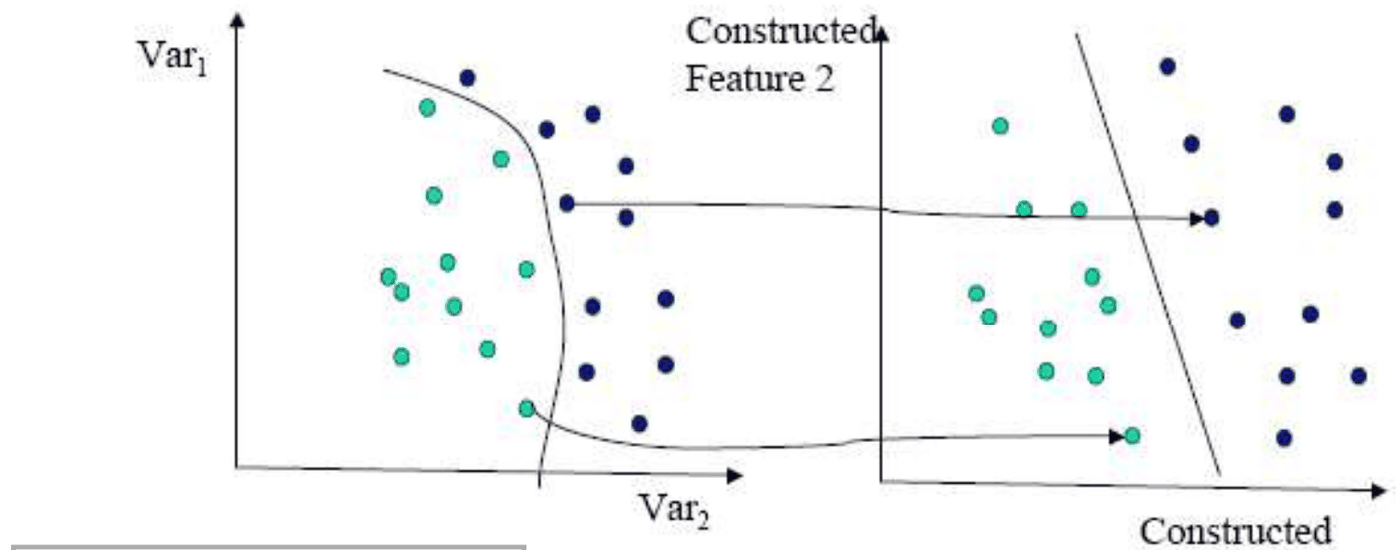
\includegraphics[width=0.91\linewidth,height=0.42\textheight,keepaspectratio]{images/13-svm_mapping.png}
\caption{A function \(\Phi(\mathbf{x})\) maps the data into a space where
they are linearly separable (recall the LBE of linear models).}
\end{figure}

\begin{boxexample}{From \(\mathbb{R}^2\) to \(\mathbb{R}^3\)}

With \(\Phi: \mathbb{R}^2 \to \mathbb{R}^3\),
\((x_1, x_2)^T \mapsto (x_1^2, \sqrt{2}x_1x_2, x_2^2)^T\)
(second-degree monomials), two classes separated by an ellipse in the
input space become separable by a \textbf{plane} in the feature space.

\end{boxexample}

\begin{figure}[htbp]
\centering
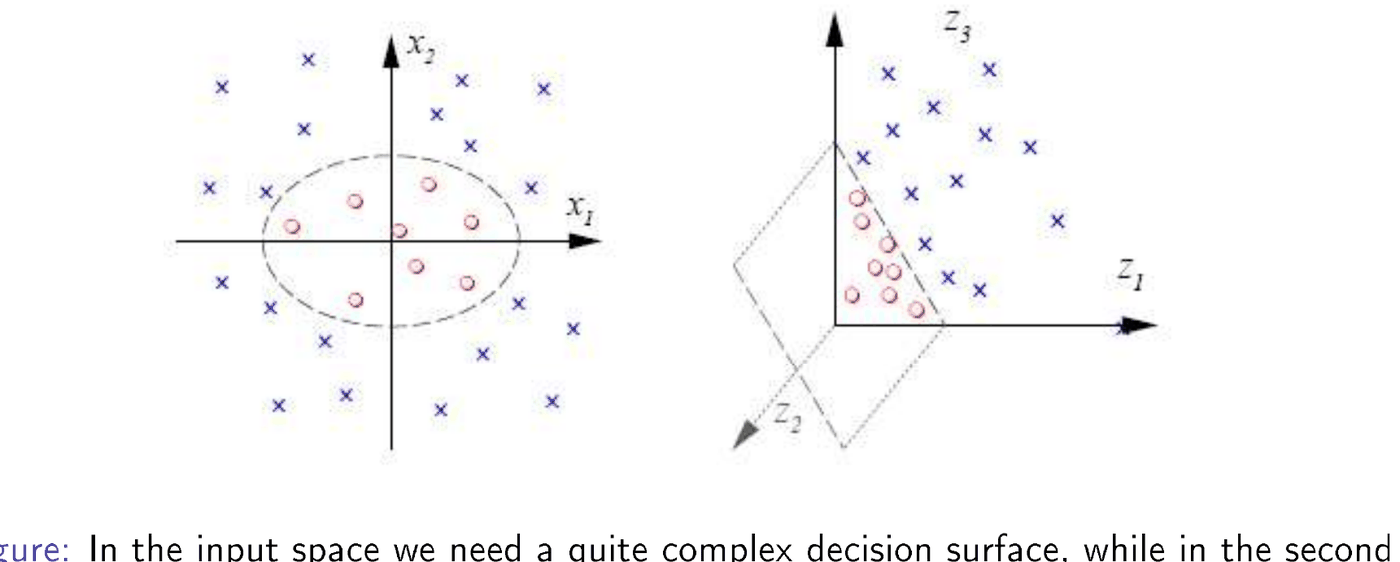
\includegraphics[width=0.89\linewidth,height=0.42\textheight,keepaspectratio]{images/13-svm_esempio-phi.png}
\caption{In the input space a complex surface is needed; in the space of
second-degree monomials a linear function is enough.}
\end{figure}

The mapping in the example is built on purpose to solve the problem
(the features correspond to ellipsoids in the original space). But
finding the ``best'' transformation \textbf{is not automatic} (unless
there is prior knowledge); general transformations are often used.
\textbf{The choice of \(\Phi\) is the critical point of SVMs.}

\subsection{High-dimensional feature
spaces}\label{spazi-di-feature-ad-alta-dimensione}

The procedure is: (1) non-linear mapping of the patterns into a
high-dimensional feature space (by \textbf{Cover's theorem}, the
patterns are linearly separable there with high probability); (2)
search for the optimal hyperplane in the feature space.

But we know that very large feature spaces (wide basis expansions) can
be \textbf{computationally infeasible} and lead to \textbf{overfitting}
without controlling the size of the space and the complexity of the
classifier. The \textbf{kernel approach} makes it possible to handle
the feature space \textbf{implicitly}, in a regularised context (where
it is the \textbf{margin} that controls complexity, not the dimension
of the input space).

With \(\Phi: \mathbb{R}^{m_0} \to \mathbb{R}^{m_1}\), the training set
becomes \(\{(\Phi(\mathbf{x}_i), d_i)\}\) and the hyperplane
\(\mathbf{w}^T\Phi(\mathbf{x}) + b = 0\). Including the bias
(\(w_0 = b\), \(\phi_0(\mathbf{x}) = 1\)), the decision surface
\(\mathbf{w}^T\Phi(\mathbf{x}) = 0\) is a \textbf{linear basis
expansion} in which the dimension of the space can be very large and
the complexity depends on the \textbf{margin}, not on the dimension.

The weight vector is
\(\mathbf{w} = \sum_i \alpha_i d_i\Phi(\mathbf{x}_i)\), and the
hyperplane becomes \[
\sum_{i=1}^{N}\alpha_i d_i\,\underbrace{\Phi^T(\mathbf{x}_i)\Phi(\mathbf{x})}_{\text{dot product}} = 0.
\] The dot product is now in the feature space, and computing
\(\Phi(\mathbf{x})\) could be intractable.

\subsection{The kernel trick}\label{il-kernel-trick}

Under certain conditions \textbf{there is no need to compute
\(\Phi(\mathbf{x})\)}, nor even to know the feature space! A function
that directly computes the dot product in the feature space is enough:

\begin{boxdefinition}{Kernel (inner product kernel)}

\[
k: \mathbb{R}^{m_0} \times \mathbb{R}^{m_0} \to \mathbb{R}, \qquad k(\mathbf{x}_i, \mathbf{x}) = \Phi^T(\mathbf{x}_i)\,\Phi(\mathbf{x}).
\] Property: it is \textbf{symmetric},
\(k(\mathbf{x}_i, \mathbf{x}) = k(\mathbf{x}, \mathbf{x}_i)\).

\end{boxdefinition}

\begin{boxexample}{The kernel of the example}

With \(\Phi(\mathbf{x}) = (x_1^2, \sqrt{2}x_1x_2, x_2^2)^T\), for
\(\mathbf{x} = (x_1, x_2)^T\) and \(\mathbf{y} = (y_1, y_2)^T\): \[
\Phi^T(\mathbf{x})\Phi(\mathbf{y}) = x_1^2y_1^2 + 2x_1x_2y_1y_2 + x_2^2y_2^2 = (x_1y_1 + x_2y_2)^2 = (\mathbf{x}^T\mathbf{y})^2 = k(\mathbf{x}, \mathbf{y}).
\] \textbf{Very important}: the dot product in the (3D) feature space
is computed \textbf{without going through the mapping}, directly in
terms of the (2D) input patterns.

\end{boxexample}

\subsection{The kernel matrix}\label{la-matrice-kernel}

The dot products between the images of the training patterns are
organised in an \(N \times N\) matrix, the \textbf{kernel matrix} (or
Gram matrix): \[
K = \{k(\mathbf{x}_i, \mathbf{x}_j)\}_{i,j=1}^N,
\] symmetric because the kernel is symmetric.

\textbf{Does every kernel function compute a dot product in some
space?} No: the property holds only for kernels that produce
\textbf{positive semidefinite} kernel matrices (\textbf{Mercer's
theorem}), i.e.\ with non-negative eigenvalues.

Closure properties: if \(k_1\) and \(k_2\) are kernels, so are
\(k_1 + k_2\), \(\alpha k_1\) (with \(\alpha > 0\)) and \(k_1 k_2\).

\subsection{SVM with kernels}\label{svm-con-kernel}

The primal in the feature space is the same as the soft margin one with
\(\Phi(\mathbf{x}_i)\) instead of \(\mathbf{x}_i\) (but \(\mathbf{w}\)
lives in the feature space, which can make the problem intractable).
The \textbf{dual}, instead, is tractable:

\begin{boxdefinition}{Dual problem in the feature space}

Find \(\{\alpha_i\}\) that maximise \[
Q(\boldsymbol{\alpha}) = \sum_{i=1}^{N}\alpha_i - \frac{1}{2}\sum_{i,j=1}^{N}\alpha_i\alpha_j d_i d_j\,\underbrace{k(\mathbf{x}_i, \mathbf{x}_j)}_{K_{ij}}
\] subject to \(\sum_i\alpha_i d_i = 0\) and \(0 \le \alpha_i \le C\).

\end{boxdefinition}

The kernel incorporates the mapping into the feature space. The
dependence on \(N\) (instead of the dimension of the space) now becomes
an \textbf{advantage}, because the feature space can have a very high
or infinite dimension.

\begin{boxabstract}{Summary of the procedure}

\begin{enumerate}
\def\labelenumi{\arabic{enumi}.}
\tightlist
\item
  We have the training set \(T = \{(\mathbf{x}_i, d_i)\}\).
\item
  The parameter \(C\) and the kernel function \(k\) are chosen.
\item
  The kernel matrix \(K\) is computed.
\item
  The optimisation problem (quadratic programming) is solved, finding
  \(\{\alpha_i\}\).
\item
  The bias \(b\) is computed from the multipliers and the kernel
  matrix.
\item
  For a new pattern \(\mathbf{x}\):
  \(\mathbf{w}^T\Phi(\mathbf{x}) = \sum_i\alpha_i d_i\,k(\mathbf{x}, \mathbf{x}_i) + b\)
  (without ever computing \(\mathbf{w}\)!), and it is classified with
  the sign.
\end{enumerate}

\textbf{Sparsity}: the solution is sparse in the \(\alpha\), because
all the multipliers of non-support vectors are zero.

\end{boxabstract}

In the test phase:
\(h(\mathbf{x}) = \operatorname{sign}\left(\sum_i\alpha_i d_i\,k(\mathbf{x}, \mathbf{x}_i) + b\right)\).
The \(\mathbf{x}_i\) (the support vectors) are stored for the test
phase: does it resemble K-NN?

\subsection{``Architectural'' view of an
SVM}\label{vista-architetturale-di-una-svm}

\begin{figure}[htbp]
\centering
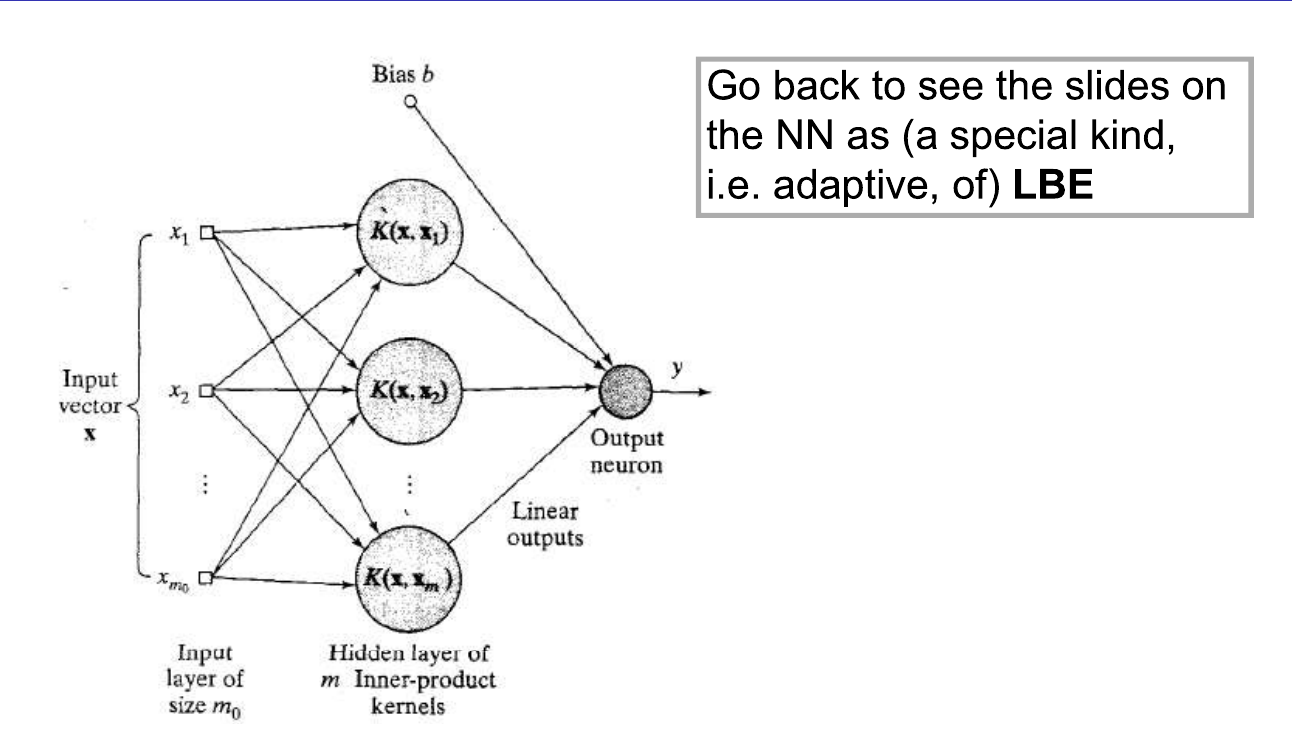
\includegraphics[width=0.66\linewidth,height=0.42\textheight,keepaspectratio]{images/13-svm_architettura.png}
\caption{``Architecture'' of an SVM: number of hidden units = number of
support vectors.}
\end{figure}

The number of ``hidden units'' is equal to the \textbf{number of
support vectors}, but they are not exactly the same units as in a
neural network: the hidden units of a network have \textbf{adaptive
free parameters}, whereas here the ``centres'' are the support vectors
themselves and the function is fixed by the kernel. It is only an
illustrative view: to be compared with neural networks (an adaptive
form of LBE) in terms of complexity control, efficiency and other
characteristics.

\subsection{Examples of kernels}\label{esempi-di-kernel}

\begin{itemize}
\tightlist
\item
  \textbf{Polynomial}:
  \(k(\mathbf{x}, \mathbf{x}_i) = (\mathbf{x}^T\mathbf{x}_i + 1)^p\),
  with \(p\) chosen by the user.
\item
  \textbf{RBF} (\emph{Radial Basis Function}, also called
  \textbf{Gaussian kernel}):
  \(k(\mathbf{x}, \mathbf{x}_i) = e^{-\frac{1}{2\sigma^2}\|\mathbf{x} - \mathbf{x}_i\|^2}\),
  with \(\sigma^2\) chosen by the user. With very ``narrow'' kernels
  (small \(\sigma\)) the response on \(\mathbf{x}_i\) is just \(d_i\)
  (it resembles 1-NN!).
\item
  \textbf{Two-layer perceptron}:
  \(k(\mathbf{x}, \mathbf{x}_i) = \tanh(\beta_0\mathbf{x}^T\mathbf{x}_i + \beta_1)\),
  with \(\beta_0 > 0\) and \(\beta_1 < 0\).
\end{itemize}

\begin{boxwarning}{Important}

For the polynomial and the RBF kernel one \textbf{always} obtains a
valid kernel (dot product), whereas for the two-layer perceptron
Mercer's theorem holds only for some choices of \(\beta_0\) and
\(\beta_1\). An RBF kernel always corresponds to a feature space of
\textbf{infinite dimension}.

\end{boxwarning}

\section{Part II --- SVM for non-linear
regression}\label{parte-ii-svm-per-la-regressione-non-lineare}

\subsection{The problem}\label{il-problema}

We have \(d = f(\mathbf{x}) + v\), with \(f\) unknown and noise \(v\)
independent of \(\mathbf{x}\). \(d\) is estimated with a linear
expansion of non-linear functions: \[
y = h(\mathbf{x}) = \mathbf{w}^T\Phi(\mathbf{x}), \qquad \mathbf{w} = (b, w_1, \dots, w_{m_1})^T, \quad \Phi(\mathbf{x}) = (1, \phi_1(\mathbf{x}), \dots, \phi_{m_1}(\mathbf{x}))^T.
\]

\subsection{\texorpdfstring{The
\(\varepsilon\)-insensitive loss}{The \textbackslash varepsilon-insensitive loss}}\label{la-loss-varepsilon-insensitive}

\[
L_\varepsilon(d, y) = \begin{cases} |d - y| - \varepsilon & \text{if } |d - y| \ge \varepsilon \\ 0 & \text{otherwise.} \end{cases}
\]

\begin{figure}[htbp]
\centering
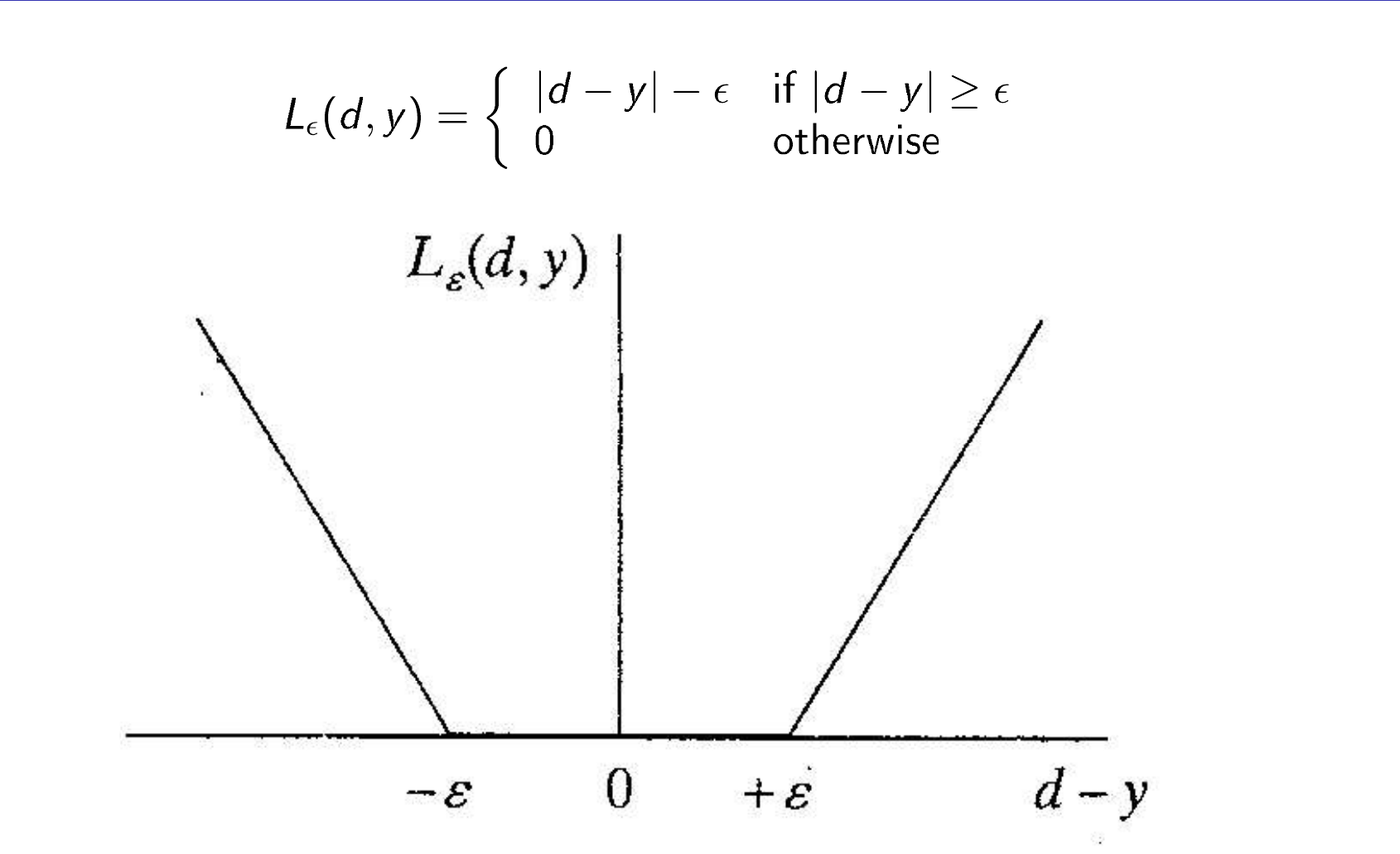
\includegraphics[width=0.54\linewidth,height=0.42\textheight,keepaspectratio]{images/13-svm_eps-loss.png}
\caption{The \(\varepsilon\)-insensitive loss.}
\end{figure}

Errors smaller than \(\varepsilon\) \textbf{cost nothing}: a
\textbf{tube} of width \(\varepsilon\) forms around the prediction, and
only the points outside the tube contribute to the loss. Again,
\textbf{only the support vectors drive the solution}: in classification
they were the points beyond the margin, here they are the points
outside the tube.

\begin{figure}[htbp]
\centering
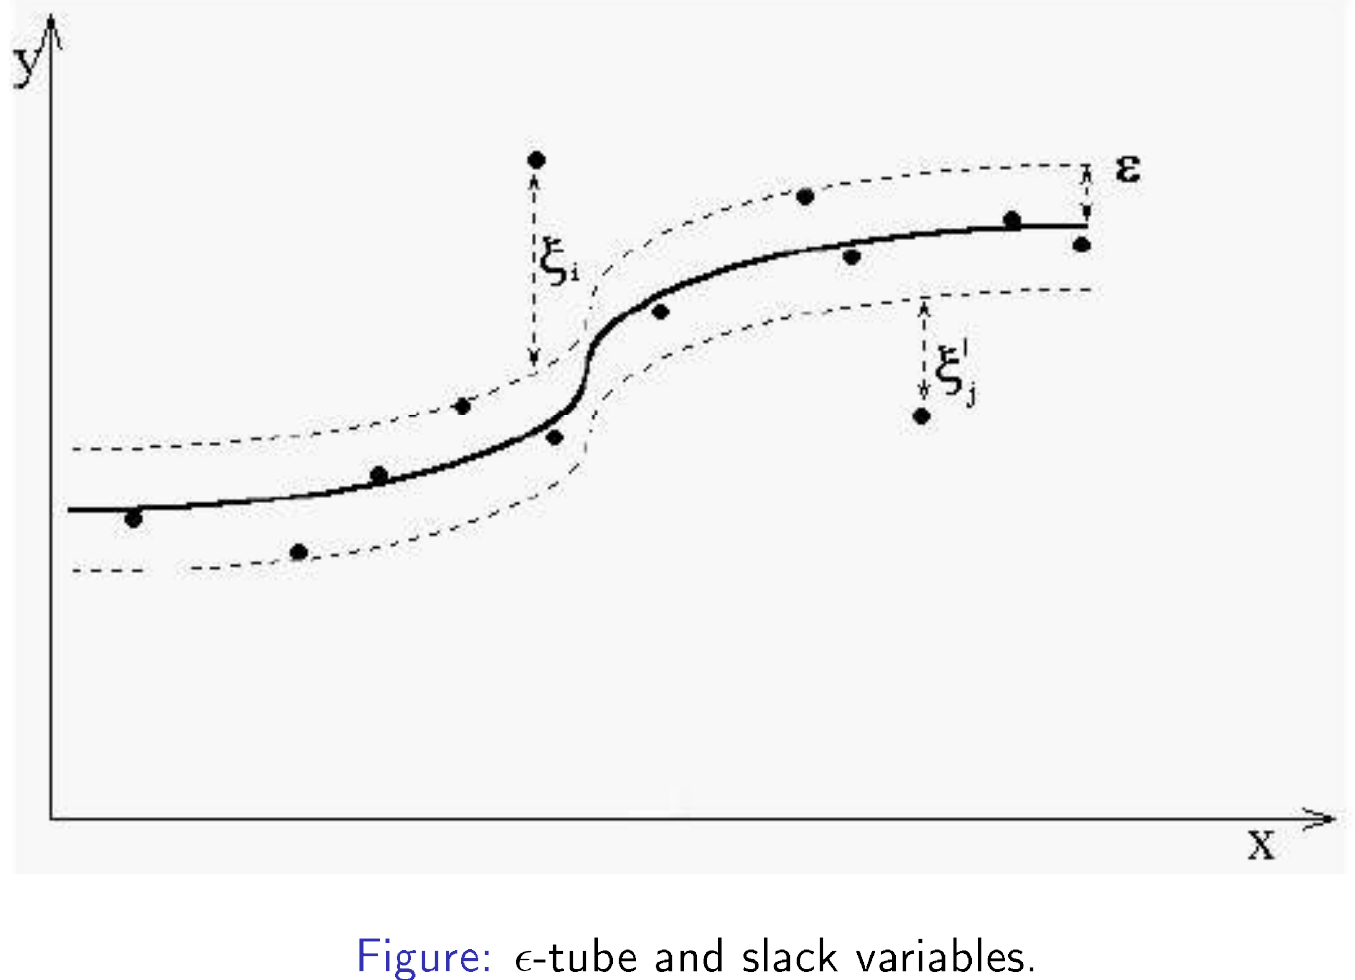
\includegraphics[width=0.60\linewidth,height=0.42\textheight,keepaspectratio]{images/13-svm_eps-tube.png}
\caption{The \(\varepsilon\) tube and the slack variables for
regression.}
\end{figure}

\subsection{Formulation}\label{formulazione}

Two sets of non-negative slack variables \(\xi_i\) and \(\xi'_i\)
(above and below the tube) are introduced: \[
-\xi'_i - \varepsilon \le d_i - \mathbf{w}^T\Phi(\mathbf{x}_i) \le \varepsilon + \xi_i.
\]

\begin{boxdefinition}{Primal problem --- SVM for regression}

Minimise \[
\Psi(\mathbf{w}, \boldsymbol{\xi}, \boldsymbol{\xi}') = \frac{1}{2}\mathbf{w}^T\mathbf{w} + C\sum_{i=1}^{N}(\xi_i + \xi'_i)
\] subject to
\(d_i - \mathbf{w}^T\Phi(\mathbf{x}_i) \le \varepsilon + \xi_i\),
\(\;\mathbf{w}^T\Phi(\mathbf{x}_i) - d_i \le \varepsilon + \xi'_i\),
\(\;\xi_i \ge 0\), \(\;\xi'_i \ge 0\).

\end{boxdefinition}

\begin{boxdefinition}{Dual problem --- SVM for regression*}

Find \(\{\alpha_i\}\) and \(\{\alpha'_i\}\) that maximise \[
Q(\boldsymbol{\alpha}, \boldsymbol{\alpha}') = \sum_{i=1}^{N}d_i(\alpha_i - \alpha'_i) - \varepsilon\sum_{i=1}^{N}(\alpha_i + \alpha'_i) - \frac{1}{2}\sum_{i,j=1}^{N}(\alpha_i - \alpha'_i)(\alpha_j - \alpha'_j)\,k(\mathbf{x}_i, \mathbf{x}_j)
\] subject to \(\sum_i(\alpha_i - \alpha'_i) = 0\) and
\(0 \le \alpha_i, \alpha'_i \le C\).

\end{boxdefinition}

From the solution: \[
\mathbf{w} = \sum_{i=1}^{N}\underbrace{(\alpha_i - \alpha'_i)}_{\gamma_i}\Phi(\mathbf{x}_i), \qquad h(\mathbf{x}) = \sum_{i=1}^{N}\gamma_i\,\Phi^T(\mathbf{x}_i)\Phi(\mathbf{x}) = \sum_{i=1}^{N}\gamma_i\,k(\mathbf{x}_i, \mathbf{x}).
\] The \textbf{support vectors} correspond to the non-zero
\(\gamma_i\).

\begin{boxabstract}{Summary for regression}

\begin{enumerate}
\def\labelenumi{\arabic{enumi}.}
\tightlist
\item
  Choose the parameters \(C\) and \(\varepsilon\).
\item
  Choose a kernel \(k\).
\item
  Compute the kernel matrix \(K\).
\item
  Solve the dual and obtain the \(\gamma_i\).
\item
  Compute the optimal bias.
\item
  The estimated function is a linear combination of dot products in a
  feature space that we can ignore:
  \(h(\mathbf{x}) = \sum_i\gamma_i\,k(\mathbf{x}_i, \mathbf{x})\).
\end{enumerate}

\end{boxabstract}

\begin{boxquestion}{What you need to know}

\begin{itemize}
\tightlist
\item
  The definition of a \textbf{maximum margin} classifier.
\item
  How maximum margin turns into a \textbf{quadratic programming}
  problem.
\item
  What QP does for us (not how it does it).
\item
  Why the SVM approximates \textbf{SRM}.
\item
  How \textbf{noisy} (non-separable) data are handled: soft margin.
\item
  How \textbf{non-linear boundaries} are obtained: kernels.
\item
  How kernels make it possible to work with very high-dimensional basis
  expansions without computing them.
\item
  How SVM for regression works (\(\varepsilon\)-insensitive loss).
\end{itemize}

\end{boxquestion}

References: Haykin, \emph{Neural Networks} (2nd ed.), ch.\ 6
(``necessary and sufficient''); Burges, \emph{A Tutorial on Support
Vector Machines for Pattern Recognition}; Schölkopf and Smola,
\emph{Learning with Kernels}; Vapnik, \emph{The Nature of Statistical
Learning Theory} and \emph{An Overview of Statistical Learning Theory}
(1999).
